\documentclass{article}
\usepackage{graphicx}
\usepackage{wrapfig}
\usepackage{subcaption}
\usepackage[margin=1in]{geometry}
\usepackage{amsmath} % or simply amstext
\usepackage{amssymb}
\usepackage{siunitx}
\usepackage{booktabs}
\usepackage[export]{adjustbox}
\newcommand{\angstrom}{\textup{\AA}}
\newcommand{\colormap}{jet}  % colorbar to use
\usepackage{cleveref}
\usepackage{booktabs}
\usepackage{gensymb}
\usepackage{float}

%BJC: potential titles (uncommented is current favorite)
%\title{The Transport Mechanisms of Polar Solutes in a Cross-linked H\textsubscript{II} Phase Lyotropic Liquid Crystal Membrane}
\title{Size, Shape and Functionality Dependence of Solute Transport Mechanisms in a Cross-linked H\textsubscript{II} Phase Lyotropic Liquid Crystal Membrane}
\author{Benjamin J. Coscia \and Michael R. Shirts} 

\begin{document}

  \graphicspath{{./figures/}}
  \maketitle

  \section{Introduction}

  We need highly selective membranes in order to perform efficient separations.

  Amphiphilic molecules are capable of self-assembling into ordered nanostructures.

  Lytropic liquid crystals are a class of amphiphilic molecules that can be cross-linked
  into mechanically strong membranes.
  \begin{itemize}
  	\item H\textsubscript{II} phase lyotropic liquid crystals have densely packed, uniform
	sized pores and have the potential to disrupt conventional membrane separation
	techniques by being selective based not only on size and charge, but on chemical
	functionality as well.
	\item Q\textsubscript{I} phase LLCs consist of a tortuous network of 3D interconnected
	pores.
  \end{itemize}

  We can only learn so much from experiment. MD can give us mechanistic insights with
  atomistic resolution so that we can intelligently design new membranes for 
  solute-specific separations.

  In our previous work, we studied the transport of 20 small polar molecules
  in an H\textsubscript{II} phase LLC membrane. 

  Unfortunately, the timescales that we can simulate with MD are insufficient to be
  able to predict macroscopic transport properties traditionally used to characterize
  membranes in the lab.

  % review of techniques for predicting long time scale behavior

  In this work, we have determined the transport mechanisms and macroscopic
  transport properties exhibited by a number of polar solutes with varying size,
  chemical functionality and hydrophilic character.
  \begin{itemize}
	\item Many of the separations we are interested in involve polar organic 
	compounds.
  \end{itemize} 

  We have compared our calculated diffusion coefficients with experimental
  measurements made using DOSY NMR. 

  \section{Methods}

  \subsection{Molecular Dynamics Simulations}
  
  \subsubsection*{System Setup}

  There is a broad range of water concentrations which will form a stable 
  H\textsubscript{II} phase with Na-GA3C11. 
  \begin{itemize}
	\item In the literature this system is typically synthesized with close
	to 10 wt \% water
    \item However, Resel et al. noted that the system is likely fully 
	hydrated with less than 7 wt \% water.
	\item We decided to test two different levels of water content: 5 and 10 wt \%
  \end{itemize} 

  We observed that water partitions into the tail region of our system and therefore
  built our initial configurations with water in both regions close to the expected
  equilibrium value.
  \begin{itemize}
	\item There is about 2:1 water in the pores versus in the tails for the 10 wt \% system.
	\item The amount of water present in the tails may or may not be experimentally consistent
	but if we don't put it in, the results will not be thermodynamically consistent, which 
	will give issues with measurements and calculations.
	\item See supporting info for water equilibration simulation data.
	\item We adjusted the pore radius in our systems so that the right amount of water
	fits in the pores without any vacuum using \texttt{gmx solvate}.
	\item We placed water molecules in the tail region one at a time in random locations
	with short energy minimizations between insertions.
  \end{itemize}

%  We equilibrated the initial configuration using the `wet' equilibration procedure
%  described in our previous work (reference to structure paper).
  %BJC: not sure I need to go into any details describing that procedure
%  \begin{itemize}
%	\item Series of NVT simulations with force constants on carbon atoms of aromatic
%	ring in head group
%	\item Force constants reduced according to the sequence: 1000000, 3162,
%	56, 8, 3, 2, 1, 0 kJ mol$^{-1}$ nm$^{-2}$ 
%  \end{itemize}

%  We cross-linked the equilibrated solvated configuration using the cross-linking procedure
%  described in our previous work. 

  We equilibrated an initial solvated configuration before adding solutes.
  \begin{itemize}
	\item We equilibrated the initial configuration using the `wet'
	equilibration procedure described in our previous work~\cite{coscia_understanding_2019}.
	\item We cross-linked the equilibrated solvated configuration using the
	cross-linking procedure described in our previous work. 
  \end{itemize}

  We added 6 solute molecules to each pore of the equilibrated cross-linked
  configuration.
  \begin{itemize}
	\item We equally spaced each solute in the pore
	\item 6 solutes per pore provided a balance of a useful amount of data
	for generating statistics and a low degree of interaction between solutes (reference
	to supporting information to show low degree of interaction)
	\item At each insertion point we placed a randomly oriented solute molecule
	then ran a short energy minimzation.
	\item We allowed the solutes to equilibrate for 5 ns using berendsen 
	pressure control
	\item We collected transport data using long simulations, on the order of
	1 microsecond
	\item .mdp files are in the supporting information % with pressure controlled by the Parrinello-Rahman barostat.
  \end{itemize}
  
  \subsubsection*{Modeling subdiffusion}\label{method:model_sFBM}

  Solutes in our H\textsubscript{II} LLC membrane exhibit subdiffusive
  behavior, a type of anomalous diffusion. 
  \begin{itemize}
  	\item During an anomalous diffusion process, the mean squared displacement (MSD)
  	does not grow linearly with time, rather it is of the form:
	\begin{equation} 
	\langle x^2(t) \rangle = K_{\alpha}t^\alpha
	\label{eqn:msd_form}
	\end{equation} 
	where $\alpha$ is the anomalous exponent and $K_\alpha$ is the
	generalized diffusion coefficient.
	\item A value of $\alpha < 1$ indicates a subdiffusive process, while a value of
	$\alpha = 1$ and $\alpha > 0$ is characteristic of Brownian and superdiffusive
	motion respectively.
  \end{itemize}

  \noindent We calculated both the ensemble-averaged and time-averaged MSDs
  of the simulated trajectories.
  \begin{itemize}
	\item The ensemble-averaged MSD measures the displacement of a particle from its initial
	position~\cite{meroz_toolbox_2015} and can be written as
	\begin{equation}
	\langle x^2(t) \rangle = \langle x(t) - x(0) \rangle
	\label{eqn:ensemble_msd}
	\end{equation}
%	\item The average MSD calculated in this way recovers the form of
%	Equation~\ref{eqn:msd_form}. % time-averaged should recover it too for FBM 
	\item The time-averaged MSD measures the displacement between all possible time lags
	and can be written as
	\begin{equation}
	\overline{x^2(\tau)} = \dfrac{1}{T - \tau}\int_{0}^{T - \tau} (x(t + \tau) - x(t))^2 dt
	\end{equation}
	where $\tau$ is the time lag and T is the length of the
	trajectory~\cite{meroz_toolbox_2015}. 
%	\item The time-averaged MSD becomes linear in our simulations,
%	therefore we can fit a line to its slope in order to estimate the macroscopic
%	diffusivity of the particle.
	%BJC: this needs more justification. Not many people have done it
	%BJC: could also not report them as diffusivities. Comparison of total MSD
	% should give same information
	% Linear region probably exists because dwell times on the order of large lag times
	% become negligible
  \end{itemize}
  
  \noindent Three common mathematical models for modeling anomalous subdiffusion processes include 
  continuous time random walks (CTRW), fractional Brownian motion (FBM) and
  random walks on fractals (RWF).\cite{meroz_toolbox_2015}
  \begin{itemize}
    \item FBM is common in crowded, viscoelastic environments where each step comes 
    from a Gaussian distribution but is anti-correlated to its previous 
    step.~\cite{mandelbrot_fractional_1968,jeon_fractional_2010,banks_anomalous_2005}
    \item A CTRW is characterized by a distribution of hop lengths and 
    dwell times, where each each step is characterized by independent random draws from 
    each distribution.\cite{montroll_random_1965,morrin_three_2018}
    \item An RWF is imposed by a system's geometry. Systems with tortuous pathways and dead
    ends cause anti-correlated motion.\cite{meroz_toolbox_2015,neusius_subdiffusion_2008}
    \item The processes described above can happen alone or in combination.  	
  \end{itemize}
  
  \noindent We believe that solutes in the system studied here exhibit subordinated 
  fractional Brownian motion (sFBM) where the parent process is FBM and the 
  leading process is a CTRW. 
  \begin{itemize}
  	\item The ensemble-averaged MSD differs from the time-averaged MSD, which
  	is indicative of non-ergodicity, a trait inherent to CTRWs but not FBM or RWFs.~\cite{thiel_weak_2014}
  	\item We also observe non-stationary $z$-coordinate traces of each solute's
  	center of mass (COM). %BJC: figure of a z-coordinate trace in main text or in supporting info
  	\item For a pure CTRW, the time-averaged MSD should be linear.
  	~\cite{neusius_subdiffusion_2008,meroz_subdiffusion_2010}
  	\item However, a typical time-averaged solute MSD is sublinear (see supporting
  	information), which suggests that there is another underlying subdiffusive mechanism.
  	\item The hop lengths recorded after each dwell period are anti-correlated (See supporting information)
  	\item Given the viscoelastic nature of the monomers in our system, we believe
  	the hop lengths can be modeled with FBM. 
 	\item For subordinated FBM, it can be shown that
  	\begin{equation}
  	\langle x^2(t) \rangle \simeq t^{\alpha\beta}
  	\end{equation}
  	where $\alpha$ is the anomalous exponent characteristic of the leading CTRW process
  	and $\beta$ is the anomalous exponent characteristic of the parent FBM process. 
  \end{itemize}

  \noindent We can characterize a CTRW process using the parameters which describe its
  dwell time and hop length distribution.
  \begin{itemize}
	\item We used the \texttt{ruptures} python package in order to identify
	breakpoints in solute trajectories.\cite{truong_ruptures:_2018} (See Supporting Information for more
	details on chosen parameters. i.e. type of cost function, cost function penalty
	tolerance, number of dimensions used)
	\item The corresponding hop lengths and dwell times between break points were 
	used to construct empirical distributions.
	\item For solutes in our system, the distribution of hop lengths is
	well-represented by a Gaussian distribution.~\cite{metzler_random_2000,
	metzler_anomalous_2014,neusius_subdiffusion_2009}
	\item We are most interested in the standard deviation, $\sigma$, of the 
	hop length distribution.
	\item The distribution of dwell	times is expected to fit a power law (or heavy-tailed)
	distribution proportional to $t^{-1-\alpha}$.~\cite{meroz_toolbox_2015}
	\item Because we are limited to taking measurements at discrete values
	dictated by the output frequency of our simulation trajectories, we fit the
	empirical dwell times to a discrete power law distribution whose maximum
	likelihood $\alpha$ parameter we calculated by maximizing the following
	likelihood function: 
        \begin{equation}
	\mathcal{L}(\beta) = -n\text{ln}\zeta(\beta, x_{min}) -
	\beta\sum_{i=1}^{n} \text{ln}~x_i 
	\label{eqn:powerlaw_likelihood}
	\end{equation}
	where $\beta = 1 + \alpha$, $x_i$ are collected dwell time data points,
	$n$ the total number of data points, and $\zeta$ is the Hurwitz zeta function
	where $x_{min}$ is the smallest measured value of
	$x_i$.~\cite{clauset_power-law_2009} 
	\item We obtained distributions of the hop length standard deviations, $\sigma$, and
	$\alpha$ using statistical bootstrapping.\cite{efron_introduction_1994} 
  \end{itemize}
  
  \noindent FBM processes can be described using the Hurst parameter, $H$, where 
  $H = \beta/2$.
  \begin{itemize}
  	\item Brownian motion is recovered for $H = 0.5$
	\item The autocovariance function of hop lengths has the analytical form:~\cite{mandelbrot_fractional_1968}
    \begin{equation}
	\gamma(k) = \dfrac{1}{2}\bigg[|k-1|^{2H} - 2|k|^{2H} + |k+1|^{2H}\bigg]
	\label{eqn:autocovariance}
	\end{equation}
	where $k$ is the number of increments between hops.
	\item We obtained H by performing a least squares fit of Equation~\ref{eqn:autocovariance}
	to the empirically measured autocovariance function.
	\item We used statistical bootstrapping to generate a distribution of $H$ 
	values. %BJC: can provide more detail in supporting or just reference python script
  \end{itemize}

%  We generated distributions of parameters for the dwell time and hop length
%  distributions using statistical bootstrapping.
%  \begin{itemize}
%	\item For each type of distribution, we randomly selected $n$ data points from the empirical
%	distribution with replacement.
%	\item We repeated the fitting procedure described above for each of 200 bootstrap trials.
%  \end{itemize} 

%  We calculated macroscopic diffusion coefficients by simulating trajectories orders of
%  magnitude longer than our molecular simulations.
  \noindent For each solute, we simulated 10000 sFBM trajectories for 1 $\mu$s each. 
  \begin{itemize}
	\item We constructed trajectories by simulating	sequences of dwell times and correlated 
	hop	lengths generated based on parameters randomly chosen from our bootstrapped parameter
	distributions.
	\item We propagated each trajectory until the total time reached 1 $\mu$s, and truncated
	the last data point so that the total time exactly equaled 1 $\mu$s. 
    \item Valid comparisons are only possible between fixed length sFBM simulations. The
    power law dwell time behavior gives rise to the aging phenomenon, embodied by
    a decrease in MSD with measurement time.~\cite{neusius_subdiffusion_2008,metzler_anomalous_2014}
    \item We reported the MSD after 1 $\mu$s with corresponding 95 \% intervals
% Following probably better suited for supporting information, if included at all
%	\item We randomly sample Gaussian hop lengths using the
%	\texttt{numpy.random.normal} method of the \texttt{numpy} python package.
%	\item We randomly sampled dwell times from a discrete power law
%	distribution based on the recommendations of Clauset et
%	al.~\cite{clauset_power-law_2009}: 
%	\begin{equation}
%	x = \lfloor
%	(x_{min} - \tfrac{1}{2})(1 - r)^{-1/(\alpha - 1)} + \tfrac{1}{2} \rfloor
%	\label{eqn:discrete_powerlaw_draws}
%	\end{equation}
%	where $r$ is randomly drawn from a uniform distribution which we simulated
%	with \texttt{numpy.random.uniform}.
%	\item We found that thermal noise does not significantly influence the MSD and
%	therefore did not add any noise to the simulated trajectories. (See supporting info)
  \end{itemize}

%BJC: probably don't need to explain this in great detail
%  \noindent We fixed the length of each simulated trajectory so that we could compare the total
%  MSD between different solutes without the influence of the ageing phenomenon.
%  \begin{itemize}
%	\item Ageing is defined by the tendency of the average MSD to decrease
%	as the length of trajectories are increased~\cite{metzler_anomalous_2014}.
%	\item The maximum measured dwell time can be no longer than the total length
%	of a simulated trajectory. 
%	\item As measurement time or trajectory length is increased, longer dwell times
%	are incorporated into the calculation, lowering the average MSD. (See supporting
%	info for demonstration)
%	\item We can achieve consistent total MSDs with low uncertainty for
%	simulated trajectories created with a given set of parameters if we fix the
%	trajectory length (as opposed to total number of steps).  
%  \end{itemize}

  \subsubsection*{Radial Distribution Functions}

  We measured the average radial distance of each solute of interest from the pore
  centers.
  \begin{itemize}
	\item We binned the radial distances and then normalized by the volume
	of the annulus defined by the bin edges.
	\item Although the pores are often described as straight, they have a
	small degree of tortuosity which disrupts the RDF calcuation 
	\item We obtain the best RDF by constructing splines that run through the
	pore centers.
	\item We construct the splines by dividing the membrane into 20 slices
	in the $z$-direction. Within each slice, we calculate the location of 
	the pore centers based on the average location of the aromatic rings
	that make up the monomer head groups.
	\item When calculating the RDF, the radial distance from the pore center
	is based on the distance between the solute center-of-mass and the ($x$, $y$)
	coordinates of appropriate point on the spline.
  \end{itemize}

  \subsubsection*{Coordination number}

  We quantified the coordination of solutes with surrounding molecules.
  \begin{itemize}
  	\item For each frame, we counted the identities and number of
  	coordinated molecules to a given solute based on a distance cut-off. 
	\item We found that this approach is more useful than calculating the
	3D spherical radial distribution function because it gives detailed
	frame-by-frame information rather than an average. 
  \end{itemize}

  \subsection{Experimental}
  % BJC: For Greg to write if things work out
   
  \section{Results and Discussion}
  
  \subsection{Governing Mechanisms}\label{section:mechanism_overview}

  % BJC: seems right to summarize overarching mechanisms observed first
  The mechanisms which govern transport of small polar solutes in this 
  system can be broadly described based a solute's size, shape, and polarity.
  \begin{itemize}
    \item In general, solutes can move fastest in the pore center, where
    there is comparatively little resistance to diffusion. 
  	\item The well-established trend of decreasing solute mobility with 
  	size is not defied here, however we observe small solutes with lower-than-expected
  	MSDs because they spend time trapped between monomer head groups.
  	\item Additionally, planar molecules are prone to exhibiting similar
  	trapping behavior, even for large molecules whose similar sized, but flexible
  	counterparts exhibit faster diffusion.  %BJC: this is unproven
  	\item The polarity of solutes also influences a solute's ability to stay in
  	the pore center. Highly polar molecules tend to spend more time in the pore center,
  	while those with hydrophobic character tend to spend more time in the head group
  	region.
  	\item Finally, the ability to hydrogen bond offers a second trapping mechanism. 
  	Solutes that are hydrogen bond donors can donate hydrogen atoms to
  	any of the 5 oxygen atoms located on the monomer head groups. Increasing the 
  	number of hydrogen bond donating groups increases the solute's polarity causing
  	solutes to spend more time in the pore centers, but the effect can be countered
  	by excessive trapping if there many hydrogen bonds are being formed.
  	\item Overall solutes exhibit some degree of trapping, by one or a combination of the above
  	mechanisms, with anticorrelated hops between each period of immobility due to 
  	obstructions.
  \end{itemize}

  \end{itemize}
  
  We will explore these factors in greater detail in the context of 
  specific groups of molecules in the discussion that follows.

  \subsection{MSD Predictions}\label{section:msd_predictions}
  
  %BJC: focus on MD MSD results
  \noindent We calculated the MSD of each solute in the set over the course of 1$\mu$s MD simulations.  %BJC: type of MSD TBD 
  \begin{itemize}
	\item We extracted values of $\sigma$, $\alpha$ and $H$ for each solute
	and then simulated 10000 sFBM trajectories of the same length as our MD
	simulations, as described in Section~\ref{section:model_sFBM} of the Methods.
	\item The final MSDs of the sFBM trajectories are compared to those 
	calculated directly from MD simulations in Figure~\ref{fig:all_msds}. 
	\item The three sFBM parameters, calculated based on MD solute trajectories
	are presented in Table~\ref{table:simulations}.
	\item We would like to emphasize that we rely on the MD MSD values in order to
	define trends in the total MSD, while the sFBM trajectories and parameter 
	values allow us to speculate as to the reasons for the observed trends. 
	\item There is a non-negligible amount of error in the calculation of 
	each parameter which prevents us from reliably portraying our sFBM MSDs as
	reduced	uncertainty MD MSDs.
  \end{itemize}
  
  Our simulated sFBM MSDs qualitatively reproduce the MD trends.
  \begin{itemize}
    \item sFBM generally lower
    \item There are a few noticeable discrepancies.
    \item We will discuss reasons for these as we proceed with the discussion.
  \end{itemize}

  \begin{figure}
  \centering
  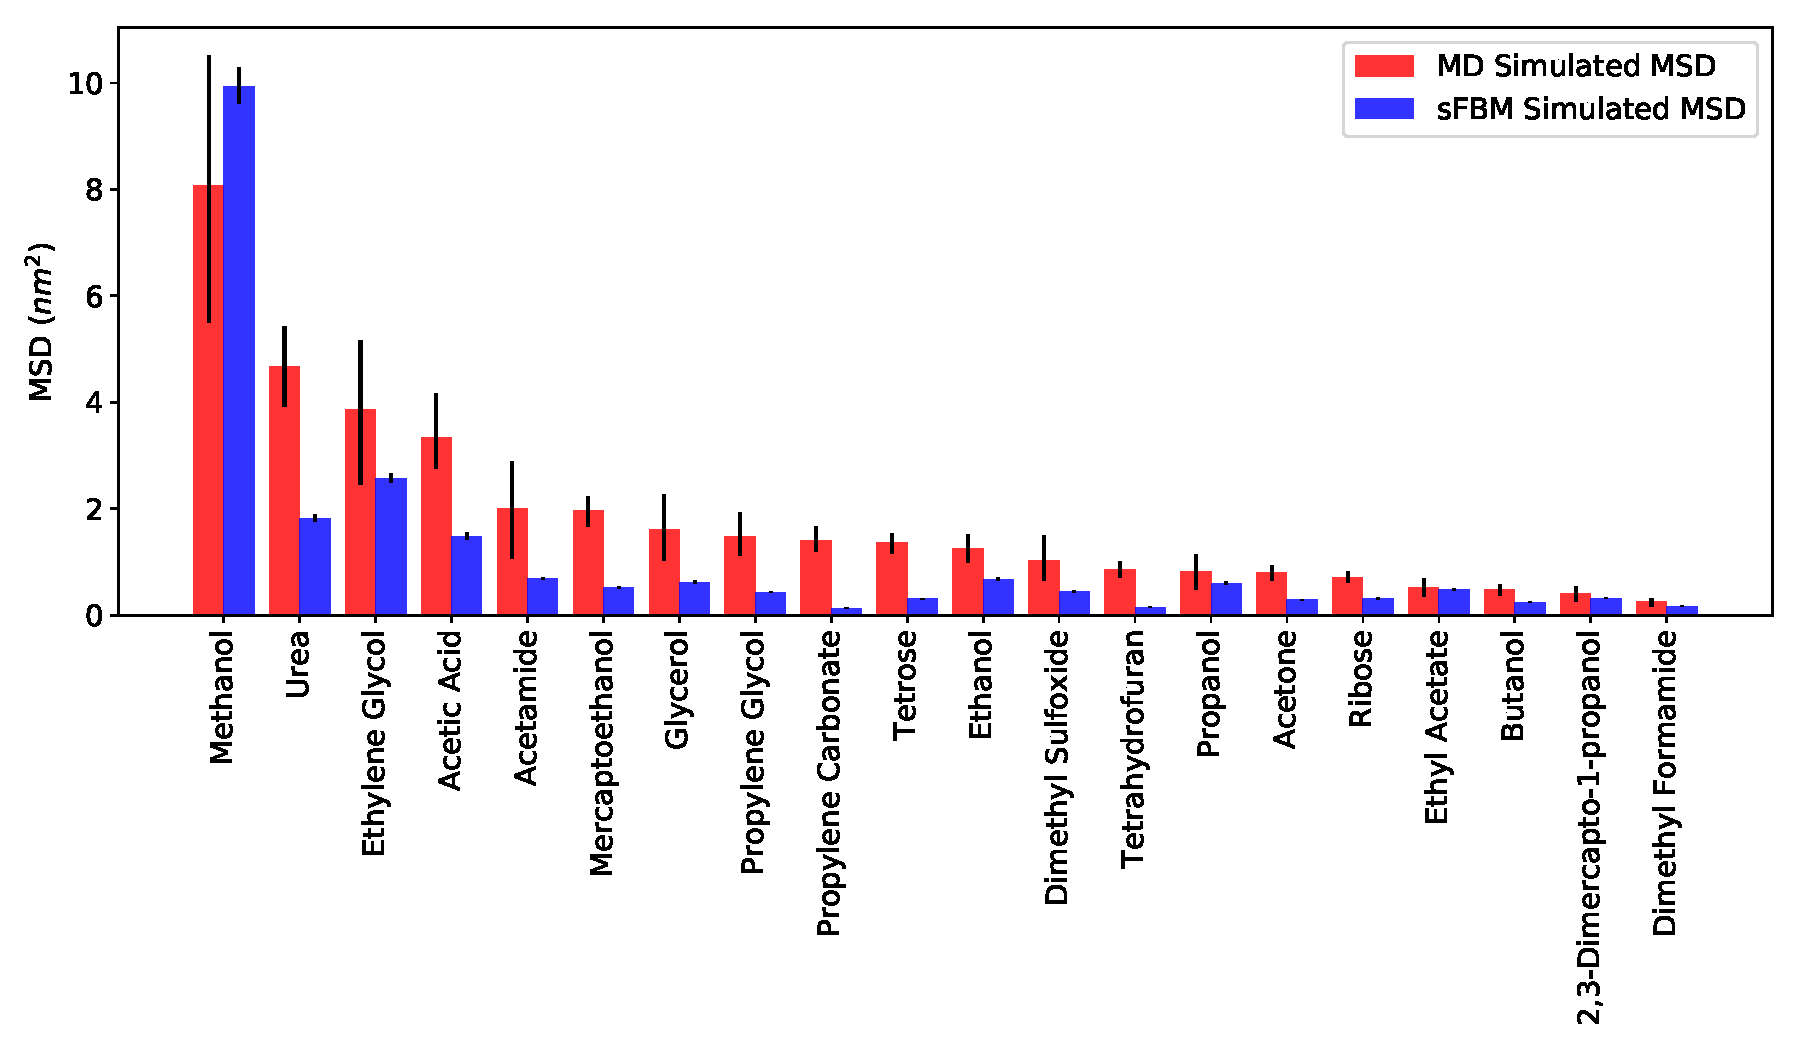
\includegraphics[width=\textwidth]{all_emsds.pdf}
  \caption{}\label{fig:all_msds}
  \end{figure}
  
  % Add MD calculated MSD to this?
  \begin{table}[h]
  \centering
  \begin{tabular}{cccc}
  \toprule
  System & $\sigma$ ($nm$) & $\alpha$ & $H$ \\
  \midrule
  Methanol & 0.46 & 0.85 & 0.40 \\
  Urea & 0.33 & 0.64 & 0.40 \\
  Ethylene Glycol & 0.35 & 0.64 & 0.36 \\
  Acetic Acid & 0.28 & 0.51 & 0.44 \\
  Mercaptoethanol & 0.30 & 0.54 & 0.26 \\
  Ethanol & 0.32 & 0.55 & 0.25 \\
  Propylene Glycol & 0.26 & 0.48 & 0.35 \\
  Glycerol & 0.23 & 0.46 & 0.37 \\
  Acetamide & 0.28 & 0.52 & 0.26 \\
  Propanol & 0.25 & 0.41 & 0.35 \\
  Acetone & 0.23 & 0.44 & 0.34 \\
  Ethyl Acetate & 0.21 & 0.41 & 0.37 \\
  Dimethyl Sulfoxide & 0.26 & 0.48 & 0.26 \\
  Tetrose & 0.24 & 0.43 & 0.30 \\
  Butanol & 0.19 & 0.41 & 0.33 \\
  Dimethyl Formamide & 0.20 & 0.39 & 0.32 \\
  2,3-Dimercapto-1-propanol & 0.20 & 0.37 & 0.35 \\
  Ribose & 0.20 & 0.40 & 0.27 \\
  Propylene Carbonate & 0.19 & 0.38 & 0.29 \\
  Tetrahydrofuran & 0.24 & 0.39 & 0.16 \\
  \bottomrule
  \end{tabular}
  \caption{We calculated values $\sigma$, $\alpha$ and $H$ from MD simulation
  trajectories and then computed the average ensemble-averaged MSD of 10000 
  simulated trajectories.}\label{table:simulations}
  \end{table}
  
  It most cases, it is easy to relate $\sigma$, $\alpha$ and $H$ to the
  simulated MSD values presented in Table~\ref{table:simulations}. 
  \begin{itemize}
  	\item Higher values of $\sigma$ indicate larger average hop lengths.
  	\item Higher values of $\alpha$ mean that there will be less sampling of 
  	long dwell times.
  	\item Values of $H$ near the Brownian limit of 0.5, indicate a lower degree
  	of anti-correlation.
  	\item All of which contribute to an overall increase in the simulated MSD
  \end{itemize}

  % BJC: figure with selected trajectories for each molecule.

  We fit a CTRW model (see Section~\ref{method:CTRW}) to these 
  trajectories and predicted macroscopic diffusion coefficients which are
  presented in Table TBD.
  \begin{itemize}
	\item We confirmed that our molecules exhibit anomalous diffusion
	by fitting a power law to the MSD curve. The exponent is less than
	1, indicative of anomalous subdiffusion.
	\item We used the decision making process given by Meroz and Sokolov
	in order to identify the appropriate subdiffusion model to use 
	based on our time series (See Section S-TBD of the Supporting info for
	more details).
	\item The motion of the solutes is non-ergodic and the steps are
	uncorrelated which tells us the system is likely well-described
	by a CTRW. 
  \end{itemize}

  % BJC: table with finalized diffusion coefficients

  \subsubsection*{The Influence of Water Content on Macroscopic Diffusion Coefficients}

  Solutes in systems with lower water content exhibit lower diffusion coefficients.
  \begin{itemize}
	\item Pores are more crowded when there is less water (show RDFs of each)
	\item Not a linear function of pore size - radius increase by x, D increases by y
	\item Larger influence on bigger molecules
  \end{itemize}

  \subsubsection{Experimental Measurements}

  % For Greg

  \subsection{Transport Mechanisms}

  In order to truly understand the molecular origins of the macroscopic
  diffusion coefficients in Section~\ref{section:D_macro}, we studied the
  microscopic interactions between solutes and the membrane that lead to the
  observed dwell time and hop distributions.
  \begin{itemize}
	\item We studied the radial distribution functions of solutes as a
	function of distance from the pore center
	\item We looked at hydrogen bonding patterns
	\item Coordination numbers
	\item Order parameters
  \end{itemize}

  The radial distribution function of each solute studied is shown in 
  Figure TBD.

  \subsubsection*{Transport of Water}

  All water molecules exhibit hop diffusion.

  Even in the center of the pore, where the density of water molecules is
  highest, individual water molecules exhibit hop diffusion as they create a
  tight hydrogen bond network.
  %TODO: the following is a hypothesis
  \begin{itemize}
	\item Water sticks to pore walls
	\item Dwell times are short
	\item Water tumbles across pore for a while until it sticks again. 
	\item Water gets caught in h-bonds with other water molecules away
	from pore center.
  \end{itemize}

  In this confined environment, the diffusion constant is x times lower than
  expected bulk diffusion coefficient of tip3p water.

  %TODO: study diffusion mechanism of water
  
  \subsubsection*{Transport of Alcohols}

  The hydroxyl functional group of alcohol molecules is a hydrogen bond donor
  and prefers to donate it's hydrogen to more strongly polarized carboxylate head
  groups.

  As alcohol groups increase in hydrophobic character, they are more inclined
  to stick to the outside edges of the pore. 
  \begin{itemize}
	\item The alkane tails prefer to stay at the edges of the pore.
	\item Radial distribution functions show peaks at pore edges, however
	smaller alcohols have high densities near the pore center. 
	\item They tend to get trapped between monomers and closer to 
	the tail region. 
	\item The entrapment is further stabilized by hydrogen bonds with
	ether oxygens connecting the monomer's alkane tails to the head groups.
	%TODO: quantify h-bonds with ether oxygens and carbonyl oxygens
  \end{itemize}

  The diffusion coefficient of simple alcohols increases as the length of 
  the alkane chain increases.
  \begin{itemize}
	\item The dwell times increase as the oily tails become more
	entrapped in monomer tails.
  \end{itemize}

  Ethylene glycol, a diol, has two hydrogen bond donor groups.
  \begin{itemize}
	\item Can hydrogen bond with same moeity.
	\item Can hydrogen bond with different moeities in the same 
	vicinity. 
	\item Dwell times tend to be shorter. If one hydroxyl group is bound
	with a hydrogen bond, the other unbound hydroxyl group may form a hydrogen bond
	elsewhere and effectively pull the other bound hydroxyl group along with it. 
  \end{itemize}

  \subsubsection*{Transport of Acetone}

  The carbonyl group of Acetone is a hydrogen bond acceptor and therefore only
  form hydrogen bonds with water molecules in the pore. 

  The hydrophobic character of the two methyl groups on acetone causes the methyl
  groups to gravitate towards the outside of the pore, while the carbonyl group
  reaches towards the pore center in order to hydrogen bond with water molecules.
  \begin{itemize}
	\item Order parameter defined between vector along carbonyl and vector extending
	from acetone COM to pore center is non-zero.
  \end{itemize} 

  \subsubsection*{Transport of Acetic Acid}

  Acetic acid, since we modeled it solely in its protonated state, has hydrogen
  bond donor and acceptor groups. 

  \subsubsection*{Transport of Ions} % probably just sodium

  Sodium ions also exhibit hop diffusion because polarized water and
  carboxylate head groups both work to neutralize its charge.
  \begin{itemize}
	\item Ions get trapped in oxygen 'cages' composed of combinations
	of water molecules, carboxylate head groups and ether oxygens connecting
	the head groups to their tails.
  	\item Interesting coordination number data
	\item Dwell time proportional to surrounding charge within coordination shell
  \end{itemize}

  \subsubsection*{Remarks}
   
  Overwhelming amount of water in 10 wt\% system makes hydrogen bonding
  competitive between head groups and water.
  %MRS: not sure what you mean above.

  \subsection{Design Suggestions}

  Water content affects pore size. Experiments to understand this could be useful.

  Separate polar molecules by creating monomers with more hydrophilic head group components.
  More incentive to dwell on walls.

  Make ions move faster by placing charges in sterically inaccessible places. 

  \section{Conclusion}

  We have examined the transport characteristics of a series of small polar
  molecules in our model of the H\textsubscript{II} phase formed by 
  Na-GA3C11.

  We calculated the macroscopic diffusion coefficients of each solute as 
  approximated by a CTRW model and validated our estimates using experimental
  DOSY NMR measurements.

  We have studied the influence of water content on the diffusion coefficients.

  We showed that hydrogen bonding between solutes and Na-GA3C11 monomers plays
  a major role in mechanism by which molecules traverse the nanopores. 

  We can use this intuition in order to modify our monomers for a specific 
  separation.
  \begin{itemize}
	\item Increase number of h-bond sites to increase selectivity towards water 
	over polar molecules
	\item Also separate acetone (things with only h-bond accepting groups) in this way
  \end{itemize}
  
 
  \section*{Supporting Information}

  Detailed explanations and expansions upon the results and procedures mentioned in
  the main text are described in the Supporting Information. This information is
  available free of charge via the Internet at http://pubs.acs.org.

  \section*{Acknowledgements}

  Molecular simulations were performed using the Extreme Science and
  Engineering Discovery Environment (XSEDE), which is supported by National
  Science Foundation grant number ACI-1548562. Specifically, it used the Bridges
  system, which is supported by NSF award number ACI-1445606, at the Pittsburgh
  Supercomputing Center (PSC). This work also utilized the RMACC Summit supercomputer,
  which is supported by the National Science Foundation (awards ACI-1532235 and
  ACI-1532236), the University of Colorado Boulder, and Colorado State
  University. The Summit supercomputer is a joint effort of the University of
  Colorado Boulder and Colorado State University.

  \clearpage

  \bibliographystyle{ieeetr}
  \bibliography{transport}

  \newpage

  \section*{TOC Graphic}

\end{document}
